\chapter{A map of variations}
\label{chapter 7}
\ifpdf
    \graphicspath{{Chapter7/Figs/}{Chapter7/Figs/PDF/}{Chapter7/Figs/}}
\else
    \graphicspath{{Chapter7/Figs/Vector/}{Chapter7/Figs/}}
\fi
This chapter provides a summary of variations, based on the results analyzed in chapter \ref{chapter 6}. The summary aims to fulfill the thesis goal outlined in section \ref{Aim of the work}, which is to define a map of variations to serve as a handbook that allows to interpret the indicator behaviors and relate a KPI change with a variation occurring in the real system. \\
The first section is dedicated to change detection, that is the step preliminary to the change identification (see introduction of chapter \ref{chapter 2}), in order to specify what system variation is possible to notice monitoring a certain KPI. \\In the second section, the process variation effects on each indicator is described and visualized through schemes representing abstractions of the KPI average behaviors, in order to outline if and how far they are fitting to give insights about the system variation extents. 
\section{Variation detection}
The goal of this section is to answer to two questions
\begin{center}
\textit{Which KPIs are able to detect a certain process variation?}\\
\vspace{3mm}
\textit{In what situation can a KPI detect a certain process variation?}
\end{center}
\begin{table}[H]
	\caption{Processing time variation detection}
	\centering
	\label{table: Processing time variation detection}
	\begin{tabular}{l c c c c l}
		\toprule
		\multirow{2}{*}{KPI} & & \multicolumn{2}{c}{Processing time} & & \multirow{2}{*}{Detection condition}\\ 
		\cmidrule(lr){3-4}
		& & Increase $\Uparrow$ & Decrease $\Downarrow$ \\
		\cmidrule{1-6}
		Input\_diff 		& & \checkmark & & & System becomes unstable \\
		Mid\_diff 			& & \checkmark & & & System becomes unstable \\
		Output\_diff 		& & \checkmark & & & System becomes unstable \\
%		\addlinespace[1em]
		Waiting\_time 		& & \checkmark & \checkmark & & \\
		Average\_Queue 		& & \checkmark & \checkmark & & \\
%		\addlinespace[1em]
		Processing\_time 	& & \checkmark & \checkmark & & \\
		Utilization 		& & \checkmark & \checkmark & & \\
%		\addlinespace[1em]	
		Blocking\_time 		& & \checkmark & \checkmark & & \\
		Blocking\_prob 		& & \checkmark & \checkmark & & \\
%		\addlinespace[1em]	
		Starving\_time 		& & \checkmark & \checkmark & & \\
		Starving\_prob 		& & \checkmark & \checkmark & & \\
		\bottomrule
	\end{tabular}
\end{table}
\begin{table}[H]
	\caption{Buffer capacity variation detection}
	\centering
	\label{table: Buffer capacity variation detection}
	\begin{tabular}{l c c c c l}
		\toprule
		\multirow{2}{*}{KPI} & & \multicolumn{2}{c}{Buffer capacity} & & \multirow{2}{*}{Detection condition}\\ 
		\cmidrule(lr){3-4}
		& & Increase $\Uparrow$ & Decrease $\Downarrow$ \\
		\cmidrule{1-6}
		Input\_diff 		& & & & & \\
		Mid\_diff 			& & & & & \\
		Output\_diff 		& & & & & \\
%		\addlinespace[1em]
		Waiting\_time 		& & \checkmark & \checkmark & & Buffer not highly unsaturated \\
		Average\_Queue 		& & \checkmark & \checkmark & & Buffer not highly unsaturated \\
%		\addlinespace[1em]
		Processing\_time 	& & & & &\\
		Utilization 		& & & & &\\
%		\addlinespace[1em]	
		Blocking\_time 		& & \checkmark & \checkmark & & Buffer not highly unsaturated \\
		Blocking\_prob 		& & \checkmark & \checkmark & & Buffer not highly unsaturated \\
%		\addlinespace[1em]	
		Starving\_time 		& & \checkmark & \checkmark & & Buffer not highly unsaturated \\
		Starving\_prob 		& & \checkmark & \checkmark & & Buffer not highly unsaturated \\
		\bottomrule
	\end{tabular}
\end{table}
Tables \ref{table: Processing time variation detection} and \ref{table: Buffer capacity variation detection} defines which KPIs and under what condition are able to detect the different process variations. They can be further summarized as follows
\begin{itemize}
\item Consecutive Cases Intervals KPIs (Input\_diff, Mid\_diff, and Output\_diff) change only if the system becomes unstable.
\item Processing\_time and Utilization KPIs change only when the system variation involves resource production capacities (i.e. processing time variations).
\item Waiting\_time, Blocking\_time, Starving\_time, and relative Stage State KPIs (Average\_Queue, Blocking\_prob, and Starving\_prob) change when both processing time or buffer capacity variations occur, but the second type of variation affects these KPIs only if the buffers (in particular the one in correspondence of the changing stage) are not too underused.
\end{itemize}
\section{Variation identification}
As in the previous section, also this one aims to answer to two questions
\begin{center}
\textit{Is a variation recognizable and distinguishable looking at how it impacts on the considered KPIs?}\\
\vspace{3mm}
\textit{Is the variation extent clearly identifiable looking at how it impacts on the considered KPIs?}
\end{center}
Therefore, this section focuses on summarizing the system variation effects on KPIs. \\
For each indicator, a description of its behavior and a brief comment on its usefulness are provided; then, six figures are attached, to help to visualize the KPI average behavior when a variation (increase or decrease) occurs, looking at stages upstream, in correspondence, and downstream the changing stage. 
\begin{figure}[H]
\centering
\includegraphics[width=0.4\textwidth]{PT_increase_CORR}
\caption{Example of scheme displaying the variation effects on a KPI in a certain stage}
\label{Example of scheme displaying the variation effects on a KPI in a certain stage}   
\end{figure}
Figure \ref{Example of scheme displaying the variation effects on a KPI in a certain stage} is an example plot, showing the behavior of Processing\_time KPI in correspondence of the changing stage when a processing time increase occurs.
\begin{itemize}
\item The black line represent the average KPI behavior \textbf{before} the variation occurs
\item The blue line represent the average KPI behavior \textbf{after} the variation has occurred, in case the system remained \textbf{stable}
\item The red line represent the average KPI behavior \textbf{after} the variation has occurred, in case the system became \textbf{unstable}
\end{itemize}
In these schemes, when one or more parameters are present on the y-axis (e.g. $\mu_{s_{CH}}'$ and $\mu_{s_{CH}}''$ in the example), they represent the value which the KPI settles around before or after the variation. If no parameters are present, the lines just show the approximate KPI behavior.\\
Moreover, in schemes, dashed arrows are used to visualize variations. Note that the arrow lengths are not exactly proportionate to actual KPI changes, but they only help to show the direction and the approximate extent of the indicator variations.\\
To simplify the dissertation, since their behaviors are very similar, KPIs and respective Stage State KPIs are discussed together. 
\newpage
\subsection{Processing time variation}
\subsubsection{Effects on Consecutive Cases Intervals KPIs}
Input\_diff, Mid\_diff, and Output\_diff are discussed together, since their behaviors are mostly similar.
CCI KPIs behave as follow:
\begin{itemize}
\item If a processing time increase occurs ($\mu_{s_{CH}}''>\mu_{s_{CH}}'$)
\begin{itemize}
\item If the system remains stable ($\mu_{s_{CH}}''<\mu_a$), CCI KPIs do not change, keeping settled around the average inter-arrival time $\mu_a$.
\item If the system becomes unstable ($\mu_{s_{CH}}''>\mu_a$), CCI KPIs increase equally in all stages, settling around the after-change mean processing time of the changing stage $\mu_{s_{CH}}''$.
\end{itemize}
\item If a processing time decrease occurs ($\mu_{s_{CH}}''<\mu_{s_{CH}}'$): CCI KPIs do not change, keeping settled around the average inter-arrival time $\mu_a$.
\end{itemize} 
\paragraph{CCI KPIs usefulness}CCI KPIs are reliable indicators of the system cycle time and, therefore, can be used to understand if the system is still stable after a variation. However, since they change their behavior exclusively when a variation makes the system unstable, it is impossible to detect a decrease in processing time (i.e. a production capacity gain) monitoring them because this variation never causes system instability. \\
Lastly, it must be added that Input\_diff of the first stage has a behavior that differs from CCI KPIs computed in any other position: since the first stage buffer is unlimited, it is always an inter-arrival time indicator, rather than a cycle time indicator.
\begin{landscape}
\begin{figure}[p]
  \centering
  \begin{subfigure}[t]{0.4\textwidth}
    \includegraphics[width=\textwidth]{CCI_KPIs_increase}
    \caption{Stages upstream $s_{CH}$}
    \label{fig:Processing time increase effects on Consecutive Cases Intervals KPIs - Stages upstream}   
  \end{subfigure}
  \begin{subfigure}[t]{0.4\textwidth}
    \includegraphics[width=\textwidth]{CCI_KPIs_increase}
    \caption{In correspondence with $s_{CH}$}
    \label{fig:Processing time increase effects on Consecutive Cases Intervals KPIs - In correspondence with}   
  \end{subfigure}
  \begin{subfigure}[t]{0.4\textwidth}
    \includegraphics[width=\textwidth]{CCI_KPIs_increase}
    \caption{Stages downstream $s_{CH}$}
    \label{fig:Processing time increase effects on Consecutive Cases Intervals KPIs - Stages downstream}   
  \end{subfigure}
  \caption{Processing time increase effects on Consecutive Cases Intervals KPIs}
  \label{fig:Processing time increase effects on Consecutive Cases Intervals KPIs}
\end{figure}
\begin{figure}[p]
  \centering
  \begin{subfigure}[b]{0.4\textwidth}
    \includegraphics[width=\textwidth]{CCI_KPIs_NOchange}
    \caption{Stages upstream $s_{CH}$}
    \label{fig:Processing time decrease effects on Consecutive Cases Intervals KPIs - Stages upstream}   
  \end{subfigure}
  \begin{subfigure}[b]{0.4\textwidth}
    \includegraphics[width=\textwidth]{CCI_KPIs_NOchange}
    \caption{In correspondence with $s_{CH}$}
    \label{fig:Processing time decrease effects on Consecutive Cases Intervals KPIs - In correspondence with}   
  \end{subfigure}
  \begin{subfigure}[b]{0.4\textwidth}
    \includegraphics[width=\textwidth]{CCI_KPIs_NOchange}
    \caption{Stages downstream $s_{CH}$}
    \label{fig:Processing time decrease effects on Consecutive Cases Intervals KPIs - Stages downstream}   
  \end{subfigure}
  \caption{Processing time decrease effects on Consecutive Cases Intervals KPIs}
  \label{fig:Processing time decrease effects on Consecutive Cases Intervals KPIs}
\end{figure}
\end{landscape}
\subsubsection{Effects on Processing\_time and Utilization KPIs}
Processing\_time KPI behaves as follows:
\begin{itemize}
\item When a processing time increase occurs ($\mu_{s_{CH}}''>\mu_{s_{CH}}'$) 
\begin{itemize}
\item In the changing stage, Processing\_time increases, keeping aligned with $\mu_{s_{CH}}''$. 
\item In other stages, Processing\_time does not change.
\end{itemize}
\item When a processing time decrease occurs ($\mu_{s_{CH}}''<\mu_{s_{CH}}'$)
\begin{itemize}
\item In the changing stage, Processing\_time decreases, keeping aligned with $\mu_{s_{CH}}''$.
\item In other stages, Processing\_time does not change.
\end{itemize}
\end{itemize}
Utilization KPI behaves as follows:
\begin{itemize}
	\item When a processing time increase occurs ($\mu_{s_{CH}}''>\mu_{s_{CH}}'$)
	\begin{itemize}
		\item If the system remains stable ($\mu_{s_{CH}}''<\mu_a$)
		\begin{itemize}
			\item In the changing stage, Utilization increases. 
			\item In other stages, Utilization does not change.
		\end{itemize}
		\item If the system becomes unstable ($\mu_{s_{CH}}''>\mu_a$)
		\begin{itemize}
			\item In the changing stage, Utilization increases. 
			\item In other stages, Utilization decreases.
		\end{itemize}
	\end{itemize}
	\item When a processing time decrease occurs ($\mu_{s_{CH}}''<\mu_{s_{CH}}'$)
	\begin{itemize}
		\item In the changing stage, Utilization decreases.
		\item In other stages, Utilization does not change.
	\end{itemize}
\end{itemize}
The variation extent of Processing\_time and Utilization are wider the larger the processing time variation is. Values taken by Utilization are limited to the range $[0,1]$.
\paragraph{Processing\_time and Utilization KPIs usefulness}
Both these KPIs give clear information regarding the resources: Processing\_time tells the absolute value of the average time needed by a resource to process a job, while Utilization shows how much a resource is exploited, comparing its processing time to the system cycle time.\\
Processing time variations directly impact on these KPIs, which turn out to be the most informative and swift-reacting among the considered indicators when this kind of change occurs.
\begin{landscape}
\begin{figure}[p]
  \centering
  \begin{subfigure}[t]{0.4\textwidth}
    \includegraphics[width=\textwidth]{PT_NOchange_UpDown}
    \caption{Stages upstream $s_{CH}$}
    \label{fig:Processing time increase effects on Processing time KPI - Stages upstream}   
  \end{subfigure}
  \begin{subfigure}[t]{0.4\textwidth}
    \includegraphics[width=\textwidth]{PT_increase_CORR}
    \caption{In correspondence with $s_{CH}$}
    \label{fig:Processing time increase effects on Processing time KPI - In correspondence with}   
  \end{subfigure}
  \begin{subfigure}[t]{0.4\textwidth}
    \includegraphics[width=\textwidth]{PT_NOchange_UpDown}
    \caption{Stages downstream $s_{CH}$}
    \label{fig:Processing time increase effects on Processing time KPI - Stages downstream}   
  \end{subfigure}
  \caption{Processing time increase effects on Processing time KPI}
  \label{fig:Processing time increase effects on Processing time KPI}
\end{figure}
\begin{figure}[p]
  \centering
  \begin{subfigure}[b]{0.4\textwidth}
    \includegraphics[width=\textwidth]{PT_NOchange_UpDown}
    \caption{Stages upstream $s_{CH}$}
    \label{fig:Processing time decrease effects on Processing time KPI - Stages upstream}   
  \end{subfigure}
  \begin{subfigure}[b]{0.4\textwidth}
    \includegraphics[width=\textwidth]{PT_decrease_CORR}
    \caption{In correspondence with $s_{CH}$}
    \label{fig:Processing time decrease effects on Processing time KPI - In correspondence with}   
  \end{subfigure}
  \begin{subfigure}[b]{0.4\textwidth}
    \includegraphics[width=\textwidth]{PT_NOchange_UpDown}
    \caption{Stages downstream $s_{CH}$}
    \label{fig:Processing time decrease effects on Processing time KPI - Stages downstream}   
  \end{subfigure}
  \caption{Processing time decrease effects on Processing time KPI}
  \label{fig:Processing time decrease effects on Processing time KPI}
\end{figure}
\end{landscape}
\begin{landscape}
\begin{figure}[p]
  \centering
  \begin{subfigure}[t]{0.4\textwidth}
    \includegraphics[width=\textwidth]{Utilization_increase_UpDown}
    \caption{Stages upstream $s_{CH}$}
    \label{fig:Processing time increase effects on Utilization KPI - Stages upstream}   
  \end{subfigure}
  \begin{subfigure}[t]{0.4\textwidth}
    \includegraphics[width=\textwidth]{Utilization_increase_CORR}
    \caption{In correspondence with $s_{CH}$}
    \label{fig:Processing time increase effects on Utilization KPI - In correspondence with}   
  \end{subfigure}
  \begin{subfigure}[t]{0.4\textwidth}
    \includegraphics[width=\textwidth]{Utilization_increase_UpDown}
    \caption{Stages downstream $s_{CH}$}
    \label{fig:Processing time increase effects on Utilization KPI - Stages downstream}   
  \end{subfigure}
  \caption{Processing time increase effects on Utilization KPI}
  \label{fig:Processing time increase effects on Utilization KPI}
\end{figure}
\begin{figure}[p]
  \centering
  \begin{subfigure}[b]{0.4\textwidth}
    \includegraphics[width=\textwidth]{Utilization_decrease_UpDown}
    \caption{Stages upstream $s_{CH}$}
    \label{fig:Processing time decrease effects on Utilization KPI - Stages upstream}   
  \end{subfigure}
  \begin{subfigure}[b]{0.4\textwidth}
    \includegraphics[width=\textwidth]{Utilization_decrease_CORR}
    \caption{In correspondence with $s_{CH}$}
    \label{fig:Processing time decrease effects on Utilization KPI - In correspondence with}   
  \end{subfigure}
  \begin{subfigure}[b]{0.4\textwidth}
    \includegraphics[width=\textwidth]{Utilization_decrease_UpDown}
    \caption{Stages downstream $s_{CH}$}
    \label{fig:Processing time decrease effects on Utilization KPI - Stages downstream}   
  \end{subfigure}
  \caption{Processing time decrease effects on Utilization KPI}
  \label{fig:Processing time decrease effects on Utilization KPI}
\end{figure}
\end{landscape}
\subsubsection{Effects on Waiting\_time and Average\_Queue KPIs}
Waiting\_time and Average\_Queue KPIs behave as follows:
\begin{itemize}
\item When a processing time increase occurs ($\mu_{s_{CH}}''>\mu_{s_{CH}}'$)
\begin{itemize}
\item If the system remains stable ($\mu_{s_{CH}}''<\mu_a$)
\begin{itemize}
\item In stages upstream and in correspondence with the changing stage, Waiting\_time and Average\_Queue increase.
\item In stages downstream the changing stage, Waiting\_time and Average\_Queue decrease.
\end{itemize}
\item If the system becomes unstable ($\mu_{s_{CH}}''>\mu_a$)
\begin{itemize}
\item In stages upstream and in correspondence with the changing stage
\begin{itemize}
\item Waiting\_time increases and settles around $LW_s$ \footnote{$LW_s$ is equal to the product of average cycle time (indicated by average Input\_diff) and the buffer capacity limit of stage $s$, $cl_s$}.
\item Average\_Queue increases and settles around the buffer capacity limit of stage $s$, $cl_s$.
\end{itemize}
\item In stages downstream the changing stage, Waiting\_time and Average\_Queue decrease towards $0$.
\end{itemize}
\end{itemize}
\item When a processing time decrease occurs ($\mu_{s_{CH}}''<\mu_{s_{CH}}'$)
\begin{itemize}
\item In stages upstream and in correspondence with the changing stage, Waiting\_time and Average\_Queue decrease.
\item In stages downstream the changing stage, Waiting\_time and Average\_Queue increase.
\end{itemize}
\end{itemize}
The variation extent of Waiting\_time and Average\_Queue in a certain stage $s$ is influenced by stage $s$ position, the processing time variation width ($|\mu_{s_{CH}}''-\mu_{s_{CH}}'|$), and the buffer capacity limits $cl_s$. It is possible to say that the variation extent is 
\begin{itemize}
\item wider the larger the processing time variation ($|\mu_{s_{CH}}''-\mu_{s_{CH}}'|$) is.
\item wider the nearer stage $s$ is with respect to the changing stage $s_{CH}$.
\item wider in stages near the changing stage $s_{CH}$, the higher the buffer capacity limits $cl_s$ are.
\item narrower in stages far from the changing stage $s_{CH}$, the higher the buffer capacity limits $cl_s$ are.
\end{itemize}
\paragraph{Waiting\_time and Average\_Queue KPIs usefulness}
Waiting\_time and Average\_Queue offer two different perspectives regarding the buffers: Waiting\_time has a job-oriented point of view, showing how much time jobs spent in buffers, while Average\_Queue is more queue-oriented, allowing to know how many jobs are on average simultaneously present in a buffer.\\
These KPIs allow to understand a processing time variation direction (increase or decrease) and its approximate size: Waiting\_time and Average\_Queue do not show the exact change extent, but high KPI changes are the clue that a big system variation is occurring in a stage.
\begin{landscape}
\begin{figure}[p]
  \centering
  \begin{subfigure}[t]{0.4\textwidth}
    \includegraphics[width=\textwidth]{WT_increase_Up}
    \caption{Stages upstream $s_{CH}$}
    \label{fig:Processing time increase effects on Waiting time KPI - Stages upstream}   
  \end{subfigure}
  \begin{subfigure}[t]{0.4\textwidth}
    \includegraphics[width=\textwidth]{WT_increase_CORR}
    \caption{In correspondence with $s_{CH}$}
    \label{fig:Processing time increase effects on Waiting time KPI - In correspondence with}   
  \end{subfigure}
  \begin{subfigure}[t]{0.4\textwidth}
    \includegraphics[width=\textwidth]{WT_increase_Down}
    \caption{Stages downstream $s_{CH}$}
    \label{fig:Processing time increase effects on Waiting time KPI - Stages downstream}   
  \end{subfigure}
  \caption{Processing time increase effects on Waiting time KPI}
  \label{fig:Processing time increase effects on Waiting time KPI}
\end{figure}
\begin{figure}[p]
  \centering
  \begin{subfigure}[b]{0.4\textwidth}
    \includegraphics[width=\textwidth]{WT_decrease_Up}
    \caption{Stages upstream $s_{CH}$}
    \label{fig:Processing time decrease effects on Waiting time KPI - Stages upstream}   
  \end{subfigure}
  \begin{subfigure}[b]{0.4\textwidth}
    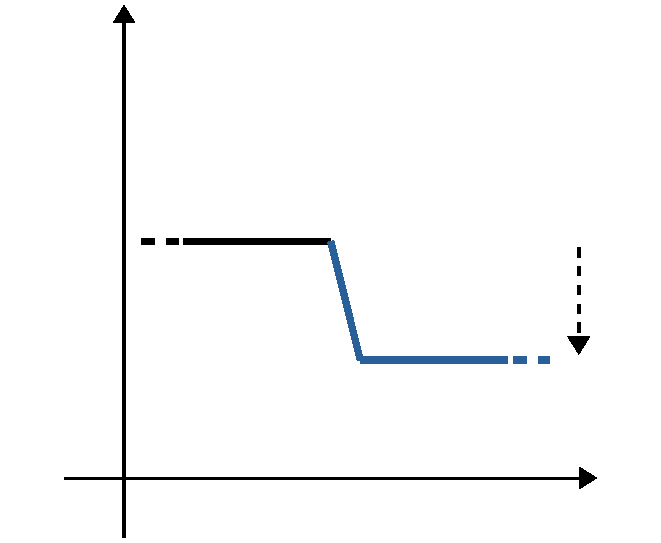
\includegraphics[width=\textwidth]{WT_decrease_CORR}
    \caption{In correspondence with $s_{CH}$}
    \label{fig:Processing time decrease effects on Waiting time KPI - In correspondence with}   
  \end{subfigure}
  \begin{subfigure}[b]{0.4\textwidth}
    \includegraphics[width=\textwidth]{WT_decrease_Down}
    \caption{Stages downstream $s_{CH}$}
    \label{fig:Processing time decrease effects on Waiting time KPI - Stages downstream}   
  \end{subfigure}
  \caption{Processing time decrease effects on Waiting time KPI}
  \label{fig:Processing time decrease effects on Waiting time KPI}
\end{figure}
\end{landscape}
\begin{landscape}
\begin{figure}[p]
  \centering
  \begin{subfigure}[t]{0.4\textwidth}
    \includegraphics[width=\textwidth]{AQ_increase_Up}
    \caption{Stages upstream $s_{CH}$}
    \label{fig:Processing time increase effects on Average Queue KPI - Stages upstream}   
  \end{subfigure}
  \begin{subfigure}[t]{0.4\textwidth}
    \includegraphics[width=\textwidth]{AQ_increase_CORR}
    \caption{In correspondence with $s_{CH}$}
    \label{fig:Processing time increase effects on Average Queue KPI - In correspondence with}   
  \end{subfigure}
  \begin{subfigure}[t]{0.4\textwidth}
    \includegraphics[width=\textwidth]{AQ_increase_Down}
    \caption{Stages downstream $s_{CH}$}
    \label{fig:Processing time increase effects on Average Queue KPI - Stages downstream}   
  \end{subfigure}
  \caption{Processing time increase effects on Average Queue KPI}
  \label{fig:Processing time increase effects on Average Queue KPI}
\end{figure}
\begin{figure}[p]
  \centering
  \begin{subfigure}[b]{0.4\textwidth}
    \includegraphics[width=\textwidth]{AQ_decrease_Up}
    \caption{Stages upstream $s_{CH}$}
    \label{fig:Processing time decrease effects on Average Queue KPI - Stages upstream}   
  \end{subfigure}
  \begin{subfigure}[b]{0.4\textwidth}
    \includegraphics[width=\textwidth]{AQ_decrease_CORR}
    \caption{In correspondence with $s_{CH}$}
    \label{fig:Processing time decrease effects on Average Queue KPI - In correspondence with}   
  \end{subfigure}
  \begin{subfigure}[b]{0.4\textwidth}
    \includegraphics[width=\textwidth]{AQ_decrease_Down}
    \caption{Stages downstream $s_{CH}$}
    \label{fig:Processing time decrease effects on Average Queue KPI - Stages downstream}   
  \end{subfigure}
  \caption{Processing time decrease effects on Average Queue KPI}
  \label{fig:Processing time decrease effects on Average Queue KPI}
\end{figure}
\end{landscape}
\subsubsection{Effects on Blocking\_time and Blocking\_prob KPIs}
Blocking\_time and Blocking\_prob KPIs behave as follows:
\begin{itemize}
\item When a processing time increase occurs ($\mu_{s_{CH}}''>\mu_{s_{CH}}'$)
\begin{itemize}
\item If the system remains stable ($\mu_{s_{CH}}''<\mu_a$)
\begin{itemize}
\item In stages upstream the changing stage, Blocking\_time and Blocking\_prob increase.
\item In stages downstream and in correspondence with the changing stage, Blocking\_time and Blocking\_prob decrease.
\end{itemize}
\item If the system becomes unstable ($\mu_{s_{CH}}''>\mu_a$)
\begin{itemize}
\item In stages upstream the changing stage
\begin{itemize}
\item Blocking\_time increases and settles around $I_s$ \footnote{$I_s$ is equal to the difference between average cycle time (indicated by Mid\_diff) and average processing time (indicated by Processing\_time) of stage $s$}.
\item Blocking\_prob increases.
\end{itemize}
\item In stages downstream and in correspondence with the changing stage, Blocking\_time and Blocking\_prob decrease and settle around $0$.
\end{itemize}
\end{itemize}
\item When a processing time decrease occurs ($\mu_{s_{CH}}''<\mu_{s_{CH}}'$)
\begin{itemize}
\item In stages upstream the changing stage, Blocking\_time and Blocking\_prob decrease.
\item In stages downstream and in correspondence with the changing stage, Blocking\_time and Blocking\_prob increase.
\end{itemize}
\end{itemize}
The variation extent of Blocking\_time and Blocking\_prob in a certain stage $s$ is influenced by stage $s$ position, the processing time variation width ($|\mu_{s_{CH}}''-\mu_{s_{CH}}'|$), and the buffer capacity limits $cl_s$. It is possible to say that the variation extent is 
\begin{itemize}
\item wider the larger the processing time variation ($|\mu_{s_{CH}}''-\mu_{s_{CH}}'|$) is
\item wider the nearer stage $s$ is with respect to the changing stage $s_{CH}$
\item wider in stages near the changing stage $s_{CH}$, the higher the buffer capacity limits $cl_s$ are 
\item narrower in stages far from the changing stage $s_{CH}$, the higher the buffer capacity limits $cl_s$ are
\end{itemize}
\paragraph{Blocking\_time and Blocking\_prob KPIs usefulness}
Blocking\_time and Blocking\_prob allow to understand how deeply stages different from the changing stage are affected by a processing time variation: Blocking\_time shows how much time jobs spend seizing a resource after being processed, because the following buffer is full, while Blocking\_prob shows how much of its available time a resource on average spends without working because a job could not leave it.\\
These KPIs allow to understand a processing time variation direction (increase or decrease) and its approximate size: Blocking\_time and Blocking\_prob do not directly indicate the exact change extent, but high KPI changes are the clue that a big system variation is occurring in a stage.
\begin{landscape}
\begin{figure}[p]
  \centering
  \begin{subfigure}[t]{0.4\textwidth}
    \includegraphics[width=\textwidth]{BT_increase_Up}
    \caption{Stages upstream $s_{CH}$}
    \label{fig:Processing time increase effects on Blocking time KPI - Stages upstream}   
  \end{subfigure}
  \begin{subfigure}[t]{0.4\textwidth}
    \includegraphics[width=\textwidth]{BT_increase_CORR}
    \caption{In correspondence with $s_{CH}$}
    \label{fig:Processing time increase effects on Blocking time KPI - In correspondence with}   
  \end{subfigure}
  \begin{subfigure}[t]{0.4\textwidth}
    \includegraphics[width=\textwidth]{BT_increase_Down}
    \caption{Stages downstream $s_{CH}$}
    \label{fig:Processing time increase effects on Blocking time KPI - Stages downstream}   
  \end{subfigure}
  \caption{Processing time increase effects on Blocking time KPI}
  \label{fig:Processing time increase effects on Blocking time KPI}
\end{figure}
\begin{figure}[p]
  \centering
  \begin{subfigure}[b]{0.4\textwidth}
    \includegraphics[width=\textwidth]{BT_decrease_Up}
    \caption{Stages upstream $s_{CH}$}
    \label{fig:Processing time decrease effects on Blocking time KPI - Stages upstream}   
  \end{subfigure}
  \begin{subfigure}[b]{0.4\textwidth}
    \includegraphics[width=\textwidth]{BT_decrease_CORR}
    \caption{In correspondence with $s_{CH}$}
    \label{fig:Processing time decrease effects on Blocking time KPI - In correspondence with}   
  \end{subfigure}
  \begin{subfigure}[b]{0.4\textwidth}
    \includegraphics[width=\textwidth]{BT_decrease_Down}
    \caption{Stages downstream $s_{CH}$}
    \label{fig:Processing time decrease effects on Blocking time KPI - Stages downstream}   
  \end{subfigure}
  \caption{Processing time decrease effects on Blocking time KPI}
  \label{fig:Processing time decrease effects on Blocking time KPI}
\end{figure}
\end{landscape}
\begin{landscape}
\begin{figure}[p]
  \centering
  \begin{subfigure}[t]{0.4\textwidth}
    \includegraphics[width=\textwidth]{BTprob_increase_Up}
    \caption{Stages upstream $s_{CH}$}
    \label{fig:Processing time increase effects on Blocking probability KPI - Stages upstream}   
  \end{subfigure}
  \begin{subfigure}[t]{0.4\textwidth}
    \includegraphics[width=\textwidth]{BTprob_increase_CORR}
    \caption{In correspondence with $s_{CH}$}
    \label{fig:Processing time increase effects on Blocking probability KPI - In correspondence with}   
  \end{subfigure}
  \begin{subfigure}[t]{0.4\textwidth}
    \includegraphics[width=\textwidth]{BTprob_increase_Down}
    \caption{Stages downstream $s_{CH}$}
    \label{fig:Processing time increase effects on Blocking probability KPI - Stages downstream}   
  \end{subfigure}
  \caption{Processing time increase effects on Blocking probability KPI}
  \label{fig:Processing time increase effects on Blocking probability KPI}
\end{figure}
\begin{figure}[p]
  \centering
  \begin{subfigure}[b]{0.4\textwidth}
    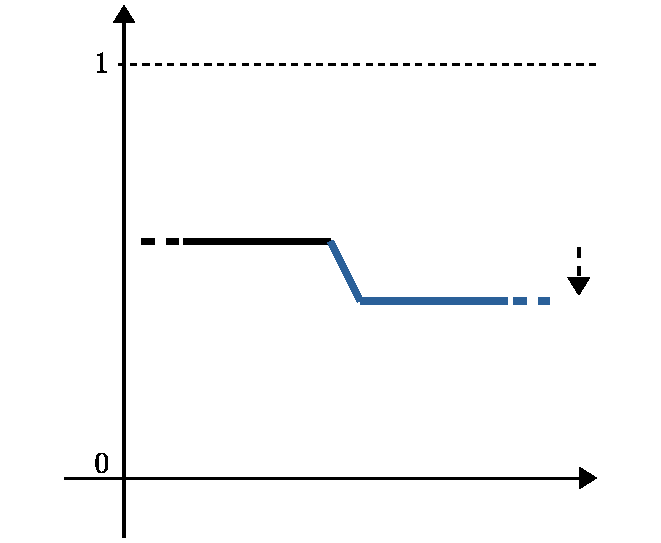
\includegraphics[width=\textwidth]{BTprob_decrease_Up}
    \caption{Stages upstream $s_{CH}$}
    \label{fig:Processing time decrease effects on Blocking probability KPI - Stages upstream}   
  \end{subfigure}
  \begin{subfigure}[b]{0.4\textwidth}
    \includegraphics[width=\textwidth]{BTprob_decrease_CORR}
    \caption{In correspondence with $s_{CH}$}
    \label{fig:Processing time decrease effects on Blocking probability KPI - In correspondence with}   
  \end{subfigure}
  \begin{subfigure}[b]{0.4\textwidth}
    \includegraphics[width=\textwidth]{BTprob_decrease_Down}
    \caption{Stages downstream $s_{CH}$}
    \label{fig:Processing time decrease effects on Blocking probability KPI - Stages downstream}   
  \end{subfigure}
  \caption{Processing time decrease effects on Blocking probability KPI}
  \label{fig:Processing time decrease effects on Blocking probability KPI}
\end{figure}
\end{landscape}
\subsubsection{Effects on Starving\_time and Starving\_prob KPIs}
Starving\_time and Starving\_prob KPIs behave as follows:
\begin{itemize}
\item When a processing time increase occurs ($\mu_{s_{CH}}''>\mu_{s_{CH}}'$)
\begin{itemize}
\item If the system remains stable ($\mu_{s_{CH}}''<\mu_a$)
\begin{itemize}
\item In stages upstream and in correspondence with the changing stage, Starving\_time and Starving\_prob decrease.
\item In stages downstream and in correspondence with the changing stage, Starving\_time and Starving\_prob increase.
\end{itemize}
\item If the system becomes unstable ($\mu_{s_{CH}}''>\mu_a$)
\begin{itemize}
\item In stages upstream and in correspondence with the changing stage, Starving\_time and Starving\_prob decrease and settle around $0$  
\item In stages downstream the changing stage
\begin{itemize}
\item Starving\_time increases and settles around $I_s$ \footnote{$I_s$ is equal to the difference between average cycle time (indicated by Mid\_diff) and average processing time (indicated by Processing\_time) of stage $s$}.
\item Starving\_prob increases 
\end{itemize}
\end{itemize}
\end{itemize}
\item When a processing time decrease occurs ($\mu_{s_{CH}}''<\mu_{s_{CH}}'$)
\begin{itemize}
\item In stages upstream and in correspondence with the changing stage, Starving\_time and Starving\_prob increase.
\item In stages downstream the changing stage, Starving\_time and Starving\_prob decrease.
\end{itemize}
\end{itemize}
The variation extent of Starving\_time and Starving\_prob in a certain stage $s$ is influenced by stage $s$ position, the processing time variation width ($|\mu_{s_{CH}}''-\mu_{s_{CH}}'|$), and the buffer capacity limits $cl_s$. It is possible to say that the variation extent is 
\begin{itemize}
\item wider the larger the processing time variation ($|\mu_{s_{CH}}''-\mu_{s_{CH}}'|$) is
\item wider the nearer stage $s$ is with respect to the changing stage $s_{CH}$
\item wider in stages near the changing stage $s_{CH}$, the higher the buffer capacity limits $cl_s$ are 
\item narrower in stages far from the changing stage $s_{CH}$, the higher the buffer capacity limits $cl_s$ are
\end{itemize}
\paragraph{Starving\_time and Starving\_prob KPIs usefulness}
Starving\_time and Starving\_prob allow to understand how deeply stages different from the changing stage are affected by a processing time variation: Starving\_time shows how much time an idle resource waits before a job seizes it, because the previous buffer is empty, while Starving\_prob shows how much of its available time a resource on average spends without working because there are no jobs to process.\\
These KPIs allow to understand a processing time variation direction (increase or decrease) and its approximate size: Starving\_time and Starving\_prob do not directly show the exact change extent, but high KPI changes are the clue that a big system variation is occurring in a stage.
\begin{landscape}
\begin{figure}[p]
  \centering
  \begin{subfigure}[t]{0.4\textwidth}
    \includegraphics[width=\textwidth]{ST_increase_Up}
    \caption{Stages upstream $s_{CH}$}
    \label{fig:Processing time increase effects on Starving time KPI - Stages upstream}   
  \end{subfigure}
  \begin{subfigure}[t]{0.4\textwidth}
    \includegraphics[width=\textwidth]{ST_increase_CORR}
    \caption{In correspondence with $s_{CH}$}
    \label{fig:Processing time increase effects on Starving time KPI - In correspondence with}   
  \end{subfigure}
  \begin{subfigure}[t]{0.4\textwidth}
    \includegraphics[width=\textwidth]{ST_increase_Down}
    \caption{Stages downstream $s_{CH}$}
    \label{fig:Processing time increase effects on Starving time KPI - Stages downstream}   
  \end{subfigure}
  \caption{Processing time increase effects on Starving time KPI}
  \label{fig:Processing time increase effects on Starving time KPI}
\end{figure}
\begin{figure}[p]
  \centering
  \begin{subfigure}[b]{0.4\textwidth}
    \includegraphics[width=\textwidth]{ST_decrease_Up}
    \caption{Stages upstream $s_{CH}$}
    \label{fig:Processing time decrease effects on Starving time KPI - Stages upstream}   
  \end{subfigure}
  \begin{subfigure}[b]{0.4\textwidth}
    \includegraphics[width=\textwidth]{ST_decrease_CORR}
    \caption{In correspondence with $s_{CH}$}
    \label{fig:Processing time decrease effects on Starving time KPI - In correspondence with}   
  \end{subfigure}
  \begin{subfigure}[b]{0.4\textwidth}
    \includegraphics[width=\textwidth]{ST_decrease_Down}
    \caption{Stages downstream $s_{CH}$}
    \label{fig:Processing time decrease effects on Starving time KPI - Stages downstream}   
  \end{subfigure}
  \caption{Processing time decrease effects on Starving time KPI}
  \label{fig:Processing time decrease effects on Starving time KPI}
\end{figure}
\end{landscape}
\begin{landscape}
\begin{figure}[p]
  \centering
  \begin{subfigure}[t]{0.4\textwidth}
    \includegraphics[width=\textwidth]{STprob_increase_Up}
    \caption{Stages upstream $s_{CH}$}
    \label{fig:Processing time increase effects on Starving probability KPI - Stages upstream}   
  \end{subfigure}
  \begin{subfigure}[t]{0.4\textwidth}
    \includegraphics[width=\textwidth]{STprob_increase_CORR}
    \caption{In correspondence with $s_{CH}$}
    \label{fig:Processing time increase effects on Starving probability KPI - In correspondence with}   
  \end{subfigure}
  \begin{subfigure}[t]{0.4\textwidth}
    \includegraphics[width=\textwidth]{STprob_increase_Down}
    \caption{Stages downstream $s_{CH}$}
    \label{fig:Processing time increase effects on Starving probability KPI - Stages downstream}   
  \end{subfigure}
  \caption{Processing time increase effects on Starving probability KPI}
  \label{fig:Processing time increase effects on Starving probability KPI}
\end{figure}
\begin{figure}[p]
  \centering
  \begin{subfigure}[b]{0.4\textwidth}
    \includegraphics[width=\textwidth]{STprob_decrease_Up}
    \caption{Stages upstream $s_{CH}$}
    \label{fig:Processing time decrease effects on Starving probability KPI - Stages upstream}   
  \end{subfigure}
  \begin{subfigure}[b]{0.4\textwidth}
    \includegraphics[width=\textwidth]{STprob_decrease_CORR}
    \caption{In correspondence with $s_{CH}$}
    \label{fig:Processing time decrease effects on Starving probability KPI - In correspondence with}   
  \end{subfigure}
  \begin{subfigure}[b]{0.4\textwidth}
    \includegraphics[width=\textwidth]{STprob_decrease_Down}
    \caption{Stages downstream $s_{CH}$}
    \label{fig:Processing time decrease effects on Starving probability KPI - Stages downstream}   
  \end{subfigure}
  \caption{Processing time decrease effects on Starving probability KPI}
  \label{fig:Processing time decrease effects on Starving probability KPI}
\end{figure}
\end{landscape}
\subsection{Buffer capacity variation}
In this subsection only Waiting\_time, Blocking\_time, Starving\_time and the respective Stage State KPIs are included. Indeed, as table \ref{table: Buffer capacity variation detection} shows, these are the only KPIs influenced by this kind of variation.
\subsubsection{Effects on Waiting\_time and Average\_Queue KPIs}
Waiting\_time and Average\_Queue KPIs behave as follows:
\begin{itemize}
\item When a buffer capacity increase occurs ($cl_s''>cl_s'$)
\begin{itemize}
\item In stages upstream the changing stage, Waiting\_time and Average\_Queue decrease.
\item In the changing stage, Waiting\_time and Average\_Queue increase.
\item In stages downstream the changing stage, Waiting\_time and Average\_Queue do not significantly change.
\end{itemize}
\item When a processing time decrease occurs ($cl_s''<cl_s'$)
\begin{itemize}
\item In stages upstream the changing stage, Waiting\_time and Average\_Queue increase.
\item In the changing stage, Waiting\_time and Average\_Queue decrease.
\item In stages downstream the changing stage, Waiting\_time and Average\_Queue do not significantly change.
\end{itemize}
\end{itemize}
The variation extent of Waiting\_time and Average\_Queue in a certain stage $s$ is influenced by stage $s$ position, and the buffer capacity variation width $|cl_{s_{CH}}''-cl_{s_{CH}}'|$. It is possible to say that the variation extent is 
\begin{itemize}
\item wider the larger the buffer capacity variation ($|\mu_{s_{CH}}''-\mu_{s_{CH}}'|$) is.
\item wider the nearer stage $s$ is with respect to the changing stage $s_{CH}$.
\item wider if the changing stage is upstream or in correspondence with the bottleneck ($s_{CH}\leqslant s_{BN}$).
\item wider the lower the before-change buffer capacity limits ($cl_s'$) are.
\end{itemize}
The last observation is linked with what is shown in table \ref{table: Buffer capacity variation detection}: if $cl_s'$ is too high, and therefore the buffers are underused and mostly unsaturated, a buffer capacity limit variation does not impact Waiting\_time and Average\_Queue, and so it cannot be detected by these KPIs. 
\paragraph{Waiting\_time and Average\_Queue KPIs usefulness}
Waiting\_time and Average\_Queue offer two different perspectives regarding the buffers: Waiting\_time has a job-oriented point of view, showing how much time jobs spent in buffers, while Average\_Queue is more queue-oriented, allowing to know how many jobs are on average simultaneously present in a buffer.\\
These KPIs allow to understand a buffer capacity variation direction (increase or decrease) and its approximate size: Waiting\_time and Average\_Queue do not show the exact change extent, but high KPI changes are the clue that a big system variation is occurring in a stage.
\begin{landscape}
\begin{figure}[p]
  \centering
  \begin{subfigure}[t]{0.4\textwidth}
    \includegraphics[width=\textwidth]{WT_Bincrease_Up}
    \caption{Stages upstream $s_{CH}$}
    \label{fig:Buffer capacity increase effects on Waiting time KPI - Stages upstream}   
  \end{subfigure}
  \begin{subfigure}[t]{0.4\textwidth}
    \includegraphics[width=\textwidth]{WT_Bincrease_CORR}
    \caption{In correspondence with $s_{CH}$}
    \label{fig:Buffer capacity increase effects on Waiting time KPI - In correspondence with}   
  \end{subfigure}
  \begin{subfigure}[t]{0.4\textwidth}
    \includegraphics[width=\textwidth]{WT_Bincrease_Down}
    \caption{Stages downstream $s_{CH}$}
    \label{fig:Buffer capacity increase effects on Waiting time KPI - Stages downstream}   
  \end{subfigure}
  \caption{Buffer capacity increase effects on Waiting time KPI}
  \label{fig:Buffer capacity increase effects on Waiting time KPI}
\end{figure}
\begin{figure}[p]
  \centering
  \begin{subfigure}[b]{0.4\textwidth}
    \includegraphics[width=\textwidth]{WT_Bdecrease_Up}
    \caption{Stages upstream $s_{CH}$}
    \label{fig:Buffer capacity decrease effects on Waiting time KPI - Stages upstream}   
  \end{subfigure}
  \begin{subfigure}[b]{0.4\textwidth}
    \includegraphics[width=\textwidth]{WT_Bdecrease_CORR}
    \caption{In correspondence with $s_{CH}$}
    \label{fig:Buffer capacity decrease effects on Waiting time KPI - In correspondence with}   
  \end{subfigure}
  \begin{subfigure}[b]{0.4\textwidth}
    \includegraphics[width=\textwidth]{WT_Bdecrease_Down}
    \caption{Stages downstream $s_{CH}$}
    \label{fig:Buffer capacity decrease effects on Waiting time KPI - Stages downstream}   
  \end{subfigure}
  \caption{Buffer capacity decrease effects on Waiting time KPI}
  \label{fig:Buffer capacity decrease effects on Waiting time KPI}
\end{figure}
\end{landscape}
\begin{landscape}
\begin{figure}[p]
  \centering
  \begin{subfigure}[t]{0.4\textwidth}
    \includegraphics[width=\textwidth]{AQ_Bincrease_Up}
    \caption{Stages upstream $s_{CH}$}
    \label{fig:Buffer capacity increase effects on Average Queue KPI - Stages upstream}   
  \end{subfigure}
  \begin{subfigure}[t]{0.4\textwidth}
    \includegraphics[width=\textwidth]{AQ_Bincrease_CORR}
    \caption{In correspondence with $s_{CH}$}
    \label{fig:Buffer capacity increase effects on Average Queue KPI - In correspondence with}   
  \end{subfigure}
  \begin{subfigure}[t]{0.4\textwidth}
    \includegraphics[width=\textwidth]{AQ_Bincrease_Down}
    \caption{Stages downstream $s_{CH}$}
    \label{fig:Buffer capacity increase effects on Average Queue KPI - Stages downstream}   
  \end{subfigure}
  \caption{Buffer capacity increase effects on Average Queue KPI}
  \label{fig:Buffer capacity increase effects on Average Queue KPI}
\end{figure}
\begin{figure}[p]
  \centering
  \begin{subfigure}[b]{0.4\textwidth}
    \includegraphics[width=\textwidth]{AQ_Bdecrease_Up}
    \caption{Stages upstream $s_{CH}$}
    \label{fig:Buffer capacity decrease effects on Average Queue KPI - Stages upstream}   
  \end{subfigure}
  \begin{subfigure}[b]{0.4\textwidth}
    \includegraphics[width=\textwidth]{AQ_Bdecrease_CORR}
    \caption{In correspondence with $s_{CH}$}
    \label{fig:Buffer capacity decrease effects on Average Queue KPI - In correspondence with}   
  \end{subfigure}
  \begin{subfigure}[b]{0.4\textwidth}
    \includegraphics[width=\textwidth]{AQ_Bdecrease_Down}
    \caption{Stages downstream $s_{CH}$}
    \label{fig:Buffer capacity decrease effects on Average Queue KPI - Stages downstream}   
  \end{subfigure}
  \caption{Buffer capacity decrease effects on Average Queue KPI}
  \label{fig:Buffer capacity decrease effects on Average Queue KPI}
\end{figure}
\end{landscape}
\subsubsection{Effects on Blocking\_time and Blocking\_prob KPIs}
Blocking\_time and Blocking\_prob KPIs behave as follows:
\begin{itemize}
\item When a buffer capacity increase occurs ($cl_s''>cl_s'$)
\begin{itemize}
\item In stages upstream the changing stage, Blocking\_time and Blocking\_prob decrease.
\item In the changing stage, Blocking\_time and Blocking\_prob increase.
\item In stages downstream the changing stage, Blocking\_time and Blocking\_prob do not significantly change.
\end{itemize}
\item When a processing time decrease occurs ($cl_s''<cl_s'$)
\begin{itemize}
\item In stages upstream the changing stage, Blocking\_time and Blocking\_prob increase.
\item In the changing stage, Blocking\_time and Blocking\_prob decrease.
\item In stages downstream the changing stage, Blocking\_time and Blocking\_prob do not significantly change.
\end{itemize}
\end{itemize}
The variation extent of Blocking\_time and Blocking\_prob in a certain stage $s$ is influenced by stage $s$ position, and the buffer capacity variation width $|cl_{s_{CH}}''-cl_{s_{CH}}'|$. It is possible to say that the variation extent is 
\begin{itemize}
\item wider the larger the buffer capacity variation ($|\mu_{s_{CH}}''-\mu_{s_{CH}}'|$) is.
\item wider the nearer stage $s$ is with respect to the changing stage $s_{CH}$.
\item wider if the changing stage is upstream or in correspondence with the bottleneck ($s_{CH}\leqslant s_{BN}$).
\item wider the lower the before-change buffer capacity limits ($cl_s'$) are.
\end{itemize}
The last observation is linked with what is shown in table \ref{table: Buffer capacity variation detection}: if $cl_s'$ is too high, and therefore the buffers are underused and mostly unsaturated, a buffer capacity limit variation does not impact Blocking\_time and Blocking\_prob, and so it cannot be detected by these KPIs. 
\paragraph{Usefulness}
Starving\_time and Starving\_prob allow to understand how deeply stages different from the changing stage are affected by a buffer capacity variation: Starving\_time shows how much time an idle resource waits before a job seizes it, because the previous buffer is empty, while Starving\_prob shows how much of its available time a resource on average spends without working because there are no jobs to process.\\
These KPIs allow to understand a buffer capacity variation direction (increase or decrease) and its approximate size: Starving\_time and Starving\_prob do not directly show the exact change extent, but high KPI changes are the clue that a big system variation is occurring in a stage.
\begin{landscape}
\begin{figure}[p]
  \centering
  \begin{subfigure}[t]{0.4\textwidth}
    \includegraphics[width=\textwidth]{BT_Bincrease_Up}
    \caption{Stages upstream $s_{CH}$}
    \label{fig:Buffer capacity increase effects on Blocking time KPI - Stages upstream}   
  \end{subfigure}
  \begin{subfigure}[t]{0.4\textwidth}
    \includegraphics[width=\textwidth]{BT_Bincrease_CORR}
    \caption{In correspondence with $s_{CH}$}
    \label{fig:Buffer capacity increase effects on Blocking time KPI - In correspondence with}   
  \end{subfigure}
  \begin{subfigure}[t]{0.4\textwidth}
    \includegraphics[width=\textwidth]{BT_Bincrease_Down}
    \caption{Stages downstream $s_{CH}$}
    \label{fig:Buffer capacity increase effects on Blocking time KPI - Stages downstream}   
  \end{subfigure}
  \caption{Buffer capacity increase effects on Blocking time KPI}
  \label{fig:Buffer capacity increase effects on Blocking time KPI}
\end{figure}
\begin{figure}[p]
  \centering
  \begin{subfigure}[b]{0.4\textwidth}
    \includegraphics[width=\textwidth]{BT_Bdecrease_Up}
    \caption{Stages upstream $s_{CH}$}
    \label{fig:Buffer capacity decrease effects on Blocking time KPI - Stages upstream}   
  \end{subfigure}
  \begin{subfigure}[b]{0.4\textwidth}
    \includegraphics[width=\textwidth]{BT_Bdecrease_CORR}
    \caption{In correspondence with $s_{CH}$}
    \label{fig:Buffer capacity decrease effects on Blocking time KPI - In correspondence with}   
  \end{subfigure}
  \begin{subfigure}[b]{0.4\textwidth}
    \includegraphics[width=\textwidth]{BT_Bdecrease_Down}
    \caption{Stages downstream $s_{CH}$}
    \label{fig:Buffer capacity decrease effects on Blocking time KPI - Stages downstream}   
  \end{subfigure}
  \caption{Buffer capacity decrease effects on Blocking time KPI}
  \label{fig:Buffer capacity decrease effects on Blocking time KPI}
\end{figure}
\end{landscape}
\begin{landscape}
\begin{figure}[p]
  \centering
  \begin{subfigure}[t]{0.4\textwidth}
    \includegraphics[width=\textwidth]{BTprob_Bincrease_Up}
    \caption{Stages upstream $s_{CH}$}
    \label{fig:Buffer capacity increase effects on Blocking prob KPI - Stages upstream}   
  \end{subfigure}
  \begin{subfigure}[t]{0.4\textwidth}
    \includegraphics[width=\textwidth]{BTprob_Bincrease_CORR}
    \caption{In correspondence with $s_{CH}$}
    \label{fig:Buffer capacity increase effects on Blocking prob KPI - In correspondence with}   
  \end{subfigure}
  \begin{subfigure}[t]{0.4\textwidth}
    \includegraphics[width=\textwidth]{BTprob_Bincrease_Down}
    \caption{Stages downstream $s_{CH}$}
    \label{fig:Buffer capacity increase effects on Blocking prob KPI - Stages downstream}   
  \end{subfigure}
  \caption{Buffer capacity increase effects on Blocking prob KPI}
  \label{fig:Buffer capacity increase effects on Blocking prob KPI}
\end{figure}
\begin{figure}[p]
  \centering
  \begin{subfigure}[b]{0.4\textwidth}
    \includegraphics[width=\textwidth]{BTprob_Bdecrease_Up}
    \caption{Stages upstream $s_{CH}$}
    \label{fig:Buffer capacity decrease effects on Blocking prob KPI - Stages upstream}   
  \end{subfigure}
  \begin{subfigure}[b]{0.4\textwidth}
    \includegraphics[width=\textwidth]{BTprob_Bdecrease_CORR}
    \caption{In correspondence with $s_{CH}$}
    \label{fig:Buffer capacity decrease effects on Blocking prob KPI - In correspondence with}   
  \end{subfigure}
  \begin{subfigure}[b]{0.4\textwidth}
    \includegraphics[width=\textwidth]{BTprob_Bdecrease_Down}
    \caption{Stages downstream $s_{CH}$}
    \label{fig:Buffer capacity decrease effects on Blocking prob KPI - Stages downstream}   
  \end{subfigure}
  \caption{Buffer capacity decrease effects on Blocking prob KPI}
  \label{fig:Buffer capacity decrease effects on Blocking prob KPI}
\end{figure}
\end{landscape}
\subsubsection{Effects on Starving\_time and Starving\_prob KPIs}
Starving\_time and Starving\_prob KPIs behave as follows:
\begin{itemize}
\item When a buffer capacity increase occurs ($cl_s''>cl_s'$)
\begin{itemize}
\item In stages upstream the changing stage, Starving\_time and Starving\_prob increase.
\item In the changing stage, Starving\_time and Starving\_prob decrease.
\item In stages downstream the changing stage, Starving\_time and Starving\_prob do not significantly change.
\end{itemize}
\item When a processing time decrease occurs ($cl_s''<cl_s'$)
\begin{itemize}
\item In stages upstream the changing stage, Starving\_time and Starving\_prob decrease.
\item In the changing stage, Starving\_time and Starving\_prob increase.
\item In stages downstream the changing stage, Starving\_time and Starving\_prob do not significantly change.
\end{itemize}
\end{itemize}
The variation extent of Starving\_time and Starving\_prob in a certain stage $s$ is influenced by stage $s$ position, and the buffer capacity variation width $|cl_{s_{CH}}''-cl_{s_{CH}}'|$. It is possible to say that the variation extent is 
\begin{itemize}
\item wider the larger the buffer capacity variation ($|\mu_{s_{CH}}''-\mu_{s_{CH}}'|$) is.
\item wider the nearer stage $s$ is with respect to the changing stage $s_{CH}$.
\item wider if the changing stage is upstream or in correspondence with the bottleneck ($s_{CH}\leqslant s_{BN}$).
\item wider the lower the before-change buffer capacity limits ($cl_s'$) are.
\end{itemize}
The last observation is linked with what is shown in table \ref{table: Buffer capacity variation detection}: if $cl_s'$ is too high, and therefore the buffers are underused and mostly unsaturated, a buffer capacity limit variation does not impact Starving\_time and Starving\_prob, and so it cannot be detected by these KPIs. 
\paragraph{Usefulness}
Starving\_time and Starving\_prob offer two different perspectives regarding the buffers: Starving\_time has a job-oriented point of view, showing how much time jobs spent in buffers, while Average\_Queue is more queue-oriented, allowing to know how many jobs are on average simultaneously present in a buffer.\\
These KPIs allow to understand a buffer capacity variation direction (increase or decrease) and its approximate size: Waiting\_time and Average\_Queue do not show the exact change extent, but high KPI changes are the clue that a big system variation is occurring in a stage.
\begin{landscape}
\begin{figure}[p]
  \centering
  \begin{subfigure}[t]{0.4\textwidth}
    \includegraphics[width=\textwidth]{ST_Bincrease_Up}
    \caption{Stages upstream $s_{CH}$}
    \label{fig:Buffer capacity increase effects on Starving time KPI - Stages upstream}   
  \end{subfigure}
  \begin{subfigure}[t]{0.4\textwidth}
    \includegraphics[width=\textwidth]{ST_Bincrease_CORR}
    \caption{In correspondence with $s_{CH}$}
    \label{fig:Buffer capacity increase effects on Starving time KPI - In correspondence with}   
  \end{subfigure}
  \begin{subfigure}[t]{0.4\textwidth}
    \includegraphics[width=\textwidth]{ST_Bincrease_Down}
    \caption{Stages downstream $s_{CH}$}
    \label{fig:Buffer capacity increase effects on Starving time KPI - Stages downstream}   
  \end{subfigure}
  \caption{Buffer capacity increase effects on Starving time KPI}
  \label{fig:Buffer capacity increase effects on Starving time KPI}
\end{figure}
\begin{figure}[p]
  \centering
  \begin{subfigure}[b]{0.4\textwidth}
    \includegraphics[width=\textwidth]{ST_Bdecrease_Up}
    \caption{Stages upstream $s_{CH}$}
    \label{fig:Buffer capacity decrease effects on Starving time KPI - Stages upstream}   
  \end{subfigure}
  \begin{subfigure}[b]{0.4\textwidth}
    \includegraphics[width=\textwidth]{ST_Bdecrease_CORR}
    \caption{In correspondence with $s_{CH}$}
    \label{fig:Buffer capacity decrease effects on Starving time KPI - In correspondence with}   
  \end{subfigure}
  \begin{subfigure}[b]{0.4\textwidth}
    \includegraphics[width=\textwidth]{ST_Bdecrease_Down}
    \caption{Stages downstream $s_{CH}$}
    \label{fig:Buffer capacity decrease effects on Starving time KPI - Stages downstream}   
  \end{subfigure}
  \caption{Buffer capacity decrease effects on Starving time KPI}
  \label{fig:Buffer capacity decrease effects on Starving time KPI}
\end{figure}
\end{landscape}
\begin{landscape}
\begin{figure}[p]
  \centering
  \begin{subfigure}[t]{0.4\textwidth}
    \includegraphics[width=\textwidth]{STprob_Bincrease_Up}
    \caption{Stages upstream $s_{CH}$}
    \label{fig:Buffer capacity increase effects on Starving prob KPI - Stages upstream}   
  \end{subfigure}
  \begin{subfigure}[t]{0.4\textwidth}
    \includegraphics[width=\textwidth]{STprob_Bincrease_CORR}
    \caption{In correspondence with $s_{CH}$}
    \label{fig:Buffer capacity increase effects on Starving prob KPI - In correspondence with}   
  \end{subfigure}
  \begin{subfigure}[t]{0.4\textwidth}
    \includegraphics[width=\textwidth]{STprob_Bincrease_Down}
    \caption{Stages downstream $s_{CH}$}
    \label{fig:Buffer capacity increase effects on Starving prob KPI - Stages downstream}   
  \end{subfigure}
  \caption{Buffer capacity increase effects on Starving prob KPI}
  \label{fig:Buffer capacity increase effects on Starving prob KPI}
\end{figure}
\begin{figure}[p]
  \centering
  \begin{subfigure}[b]{0.4\textwidth}
    \includegraphics[width=\textwidth]{STprob_Bdecrease_Up}
    \caption{Stages upstream $s_{CH}$}
    \label{fig:Buffer capacity decrease effects on Starving prob KPI - Stages upstream}   
  \end{subfigure}
  \begin{subfigure}[b]{0.4\textwidth}
    \includegraphics[width=\textwidth]{STprob_Bdecrease_CORR}
    \caption{In correspondence with $s_{CH}$}
    \label{fig:Buffer capacity decrease effects on Starving prob KPI - In correspondence with}   
  \end{subfigure}
  \begin{subfigure}[b]{0.4\textwidth}
    \includegraphics[width=\textwidth]{STprob_Bdecrease_Down}
    \caption{Stages downstream $s_{CH}$}
    \label{fig:Buffer capacity decrease effects on Starving prob KPI - Stages downstream}   
  \end{subfigure}
  \caption{Buffer capacity decrease effects on Starving prob KPI}
  \label{fig:Buffer capacity decrease effects on Starving prob KPI}
\end{figure}
\end{landscape}
%\section{KPIs from different sensor configurations}
%\begin{table}[h]
%	\caption{Timestamps necessary to compute each KPI}
%	\centering
%	\label{table: Timestamps necessary to compute each KPI}
%	\begin{tabular}{l c c c c c c}
%		\toprule
%		\multirow{2}{*}{KPI} & \multicolumn{3}{c}{Timestamps}\\ 
%		\cmidrule(lr){2-4}
%		& Timestamp\_Buffer $T_B$ & Timestamp\_Resource $T_R$ & Timestamp\_End $T_E$ \\
%		\cmidrule(lr){1-4}
%		Input\_diff & \checkmark & & \\
%		Mid\_diff & & \checkmark & \\
%		Output\_diff & & & \checkmark\\
%		Waiting\_time & \checkmark & \checkmark & \\
%		Processing\_time & & \checkmark & \checkmark \\
%		Blocking\_time & \checkmark & & \checkmark \\
%		Starving\_time & \checkmark & \checkmark & \\
%		Average\_Queue & \checkmark & \checkmark & \\
%		Utilization & & \checkmark & \checkmark \\
%		Blocking\_prob & \checkmark & & \checkmark \\
%		Starving\_prob & \checkmark & \checkmark & \\
%		\bottomrule
%	\end{tabular}
%\end{table}